\documentclass[12pt]{article}
%\usepackage{report}

\usepackage[utf8]{inputenc} % allow utf-8 input
\usepackage[T1]{fontenc}    % use 8-bit T1 fonts
\usepackage[colorlinks=true, linkcolor=blue, citecolor=blue, urlcolor=blue]{hyperref}       % hyperlinks
\usepackage{url}            % simple URL typesetting
\usepackage{booktabs}       % professional-quality tables
\usepackage{amsfonts}       % blackboard math symbols
\usepackage{nicefrac}       % compact symbols for 1/2, etc.
\usepackage{microtype}      % microtypography
\usepackage{lipsum}		% Can be removed after putting your text content
\usepackage{graphicx}
\usepackage{footnote}
\usepackage{doi}
\usepackage{comment}
\usepackage{multirow}
\usepackage{gensymb}
\usepackage{float}
\usepackage{amsmath}
\usepackage{subfig}
\usepackage{setspace}
\usepackage[skip=10pt plus1pt, indent=30pt]{parskip}
\usepackage[top=1.5in, bottom=1.5in, left=1in, right=1in]{geometry}
\usepackage{titlesec}
\begin{document}

% Adjust section heading size
\titleformat{\section}{\large\bfseries}{\thesection}{0.5em}{}

% Adjust subsection heading size
\titleformat{\subsection}{\large\bfseries}{\thesubsection}{1em}{}

\begin{titlepage}
    \centering
    
\includegraphics[width=2.3cm]{crest.jpg}\par
    \vspace{1cm}
    {\scshape\Large Department of Physics and Astronomy \par}
    \vspace{1cm}
    {\scshape\Large The University of Southampton \par}
    \vspace{1cm}
    \vspace{1cm}
    {\huge\bfseries Parameter space of the Inert Two Higgs Doublet Model (i2HDM) for Dark Matter discovery\par}
    \vspace{1cm}
    {\Large Ong Chin Phin (Linus) \par}
    \vspace{1cm}
    {\Large Student ID: 33184747 \par}
    \vfill
    {\large November 2024 \par}
\end{titlepage}

%\maketitle
\newpage
\tableofcontents
\thispagestyle{empty}

\newpage
\thispagestyle{empty}
\begin{abstract}
abstract here
\end{abstract}

\newpage
\twocolumn

\onehalfspacing
\setcounter{page}{1}
\section{Introduction}
\label{sec:introduction}
There have been strong evidence for Dark Matter (DM) over the years; Gravitational lensing, %etc, etc, add more example + source 
Although there have been recent alternative theories for the non-existance of DM \cite{Gupta_2023, Gupta_2024}, we nonetheless will continue expanding on 

Dark matter has to be neutral, colourless (lacking colour charge), non-baryonic, long-lived (DM life exceeds the age of the Universe) and massive (non-relativistic) \cite{ZACEK_2007, DeLuca2018, gondolo2004introductionnonbaryonicdarkmatter}. However, none of the SM particles fit the description perfectly - the neutrino is the closest, however it is not massive. The low mass of the neutrino causes them to move at relativistic speeds, which then do not allow the formation of large scale structures. The neutrino inspired the development a group of hypothetical particles called WIMPs (Weakly Interacting Massive Particles). Other than WIMPs, there are many models that were developed to search for DM. There are many models, but the Inert Two-Higgs Doublet Model (i2HDM) will be the model of focus in this work. 

The Higgs boson is responsible for giving masses to the $W^+, W^-$ and $Z_0$ bosons. This is done via the Higgs mechanism. The Higgs mechanism is as follows.
The Higgs doublet before electroweak symmetry breaking (EWSB), $\Phi_H$ is:
\begin{equation}
    \Phi_H =
    \begin{pmatrix}
        {\phi_1 + i\phi_2} \\
        {\phi_3 + i\phi_4}
    \end{pmatrix}
\end{equation}

%A more accurate description of the Higgs mechanism is the moving around of the degrees of freedom \cite{lyre2008does}.
This consists of 4 (real) degrees of freedom. Via the Higgs mechanism, the first 2 degrees of freedom are "given" as the mass of the $W^+$ and $W-$ boson ($\phi_1 + i\phi_2$ is the longitudinal component of $W^\pm$), whereas the third is the mass of the $Z_0$ boson. The Higgs field has one last degree of freedom ($\phi_4$), which, after symmetry breaking (when the degrees of freedom are lost to the other baryons) of the Higgs potential function is: 
\begin{equation}
    \Phi_H = \frac{1}{\sqrt{2}}
    \begin{pmatrix}
        {0} \\
        {v + H}
    \end{pmatrix}
\end{equation}

Here $v$ is the vacuum expectation value (VEV) of the Higgs potential. The Higgs potential is a function known as a Mexican hat, and the symmetry breaking allows the Higgs potential to acquire a VEV.

\begin{equation}
    \braket{\Phi} = \frac{1}{\sqrt{2}}
    \begin{pmatrix}
        0\\
        v
    \end{pmatrix}
\end{equation}

The Higgs mechanism can be described simply as the mechanism that gives the baryons we know today their masses\footnote{Fermions get their masses via Yukawa coupling with the Higgs field $\Phi$}.

The aim of this paper is to discover and perform analysis for the parameter space of the model, as a revision of the work done in \cite{Belyaev:2016lok}. In section \ref{sec:i2HDM} we introduce the i2HDM model in more detail, in Section \ref{sec:methodology} we introduce the tools used and how the parameters are fixed/scanned, in Section \ref{sec:results} the results are presented followed by an analysis in Section \ref{sec:analysis}. Finally, there is the conclusion which is in Section \ref{sec:conclusion}.

\section{Inert Two Higgs Doublet Model (i2HDM)}
\label{sec:i2HDM}
In the i2HDM, we propose two doublets, $\Phi_1$, $\Phi_2$ - where the first doublet is active and second doublet is inert. The latter does not share its degrees of freedom with other particles (or, it does not couple to fermions via Yukawa interactions \cite{Belyaev_2022}), and has no VEV; unlike the former which is just the SM Higgs doublet, which has a VEV. We can invoke a new set of particles arising from $\Phi_2$- $h^\pm, h_1,$ and $h_2$, where $m_{h_1} < m_{h_2}$ and $m_{h_1} < m_{h^\pm}$. The lightest particle, $h_1$ is the DM candidate particle.

As mentioned in the Introduction (Section \ref{sec:introduction}), i2HDM is an extension of SM that introduces new scalar particles that could be candidates for DM.

The field, along with its Hermitian conjugate is:
\begin{align}
    &\Phi_2 = \frac{1}{\sqrt{2}}
        \begin{pmatrix}
            {\sqrt{2}h^+} \\
            {h_1 + ih_2 }
        \end{pmatrix}&
    &\Phi_2^\dagger = \frac{1}{\sqrt{2}} 
        \begin{pmatrix}
            {\sqrt{2}h^-} \\
            {h_1 - ih_2 }
        \end{pmatrix}
\end{align} 

The (scalar) potential is expressed as:
\begin{equation}
    \begin{split}
        V(\Phi_1, \Phi_2) =& -m_1^2(\Phi_1^\dagger\Phi_1) - m_2^2(\Phi_2^\dagger\Phi_2)\\ 
        &+ \lambda_1(\Phi_1^\dagger\Phi_1)^2 + \lambda_2(\Phi_2^\dagger\Phi_2)^2 \\
        &+ \lambda_3(\Phi_1^\dagger\Phi_1)(\Phi_2^\dagger\Phi_2) \\
        &+ \lambda_4(\Phi_2^\dagger\Phi_1)(\Phi_1^\dagger\Phi_2)\\ 
        &+ \frac{\lambda_5}{2}[(\Phi_1^\dagger\Phi_2)^2 + (\Phi_2^\dagger\Phi_1)^2]
        \end{split}
        \label{eq:higgs_potential}
\end{equation}

Where:
\begin{itemize}
    \item $\Phi_1$ represents the active doublet
    \item $\Phi_2$ represents the inert doublet
    \item $m_1$ is the term which determines the mass of the Higgs boson and symmetry breaking\footnote{The negative sign in the first term of Equation \ref{eq:higgs_potential} makes the first term a potential with negative slope, which introduces spontaneous symmetry breaking and gives the active Higgs doublet the VEV.}
    \item $m_2$ is the mass term of the inert Higgs doublet (which helps determine the masses of the extra particles, $h_1$, $h_2$ and $h_\pm$)
    \item $\lambda_{1, 2}$ are self coupling terms of the doublets. $\lambda_1$ determines the mass of the Higgs boson and $\lambda_2$ determine the 
    \item $\lambda_{3, 4, 5}$ are the coupling terms of doublet interaction
\end{itemize}
Furthermore, we impose additional parametrisation in terms of mass differences that allow better visualisation of parameter space \cite{Belyaev_2022}, the reason which will be prevalent in the next sections when considering constrains:
\begin{align}
\label{eq:mass_diff_1}
    \Delta m^{0} = m_{h_2} - m_{h^\pm},\\
    \Delta m^1 = m_{h_2} - m_{h_1},\\
    \Delta m^+ = m_{h^\pm} - m_{h_1}
\end{align}

\subsection{The Parameter Space and its Constraints}
We have four parameters to scan across: $m_{h_1}$, $\Delta m^0$, $\Delta m^+$ and $\lambda_{345}$ (with $\lambda_2 = 1$). This will be a random scan of the parameter space, done with the software \verb|microOMEGAS|. Constraints defined in Section \ref{sec:constraints} are applied to the data sets to determine parameter space.
\label{sec:constraints}
\subsubsection{Constraints from vacuum stability and permeability}
First of all, we need to ensure that the potential is bounded from below to ensure stability \cite{Deshpande:1977rw}:
\begin{equation}
    \begin{split}
    \lambda_1>0,& \qquad
    \lambda_2>0, \qquad
    \lambda_3> -2 \sqrt{ \lambda_1 \lambda_2}, \\
    &\lambda_3 + \lambda_4 - |\lambda_5| > -2 \sqrt{ \lambda_1 \lambda_2}.
    \end{split}
    \label{eq:potential_stability}
\end{equation}
We can describe the parameter space of the i2HDM as \cite{Belyaev:2016lok}:
\begin{equation}
    \begin{split}
        m_{h_1}, \qquad m_{h_2} > m_{h_1}, \qquad m_{h^\pm} > m_{h_1}, \\
        \lambda_2 > 0, \qquad \lambda_{345} > -2\sqrt{\lambda_1 \lambda_2}
    \end{split}
\end{equation}

Where $m_{h_1}$, $m_{h_2}$ and $m_{h^\pm}$ are the masses of the 2 neutral and 2 charged inert scalars. This is to ensure that the Higgs potential is bounded from below and has a neutral, non-charge breaking vacuum, which is only satisfied if:
\begin{equation}
    \lambda_4 - |\lambda_5| < 0
\end{equation}

One could evaluate the masses of these physical scalars \cite{Belyaev:2016lok}:
\begin{align}
    \label{eqn:scalar_equations}
    &m_{Higgs}^2 = 2\lambda_1v^2 = 2m^2_1,\\
    &m_{h_\pm} = \frac{1}{2}\lambda_3v^2-m^2_2 \\
    \label{eqn:massdmscalar}
    &m_{h_1}^2 = \frac{1}{2}(\lambda_3 + \lambda_4 - |\lambda_5|)v^2 - m_2^2\\
    &m_{h_2}^2 = \frac{1}{2}(\lambda_3 + \lambda_4 + |\lambda_5|)v^2 - m_2^2 > m^2_{h_1}
\end{align}

and the mass differences: 
\begin{align}
    &m_{h_2}^2 - m_{h_1}^2 =  |\lambda_5|v^2, \\
    &m_{h_\pm}^2 - m_{h_2}^2 = -\frac{1}{2}(\lambda_4 - |\lambda_5|)v^2
\end{align}

$m_{h_1}$, $m_{h_2}$, $m_{h_\pm}$ and $\lambda_{345}$ ($\lambda_3 + \lambda_4 + \lambda_5$) are the main parameters of the study. $\lambda_{345}$ is an important parameter as it is involved in the $H\rightarrow h_1,h_1$ and $h_1,h_1 \rightarrow H$ (written in short as $Hh_1h_1$) interaction vertex. $\lambda_1$ is not a free parameter as it can be evaluated via the Higgs boson mass and the VEV. $\lambda_2$ is not considered at tree level\footnote{lowest-order approximation in perturbation theory, where Feynman diagrams do not include loops (closed paths)}; it only governs self interaction of the inert Higgs doublet, does not affect physical observables, and the DM candidate $h_1$ is only dependent on $\lambda_3$, $\lambda_4$ and $\lambda_5$ (Equation \ref{eqn:massdmscalar}). While $\lambda_2$ does not appear explicitly in the relevant interactions, it indirectly contributes to vacuum stability, ensuring a consistent and physically viable model.

In addition to that, we consider constraints due to symmetry breaking. We impose that, from \cite{Belyaev:2016lok, Ginzburg2010}:
For $|R| < 1$,
\begin{equation}
    m_{h_1}^2 > 0
\end{equation}
And for $R>1$, 
\begin{equation}
    \label{eqn:R>1}
    m_{h_1}^2 > (R-1) \sqrt{\lambda_1\lambda_2} v^2
\end{equation}

Where:
\begin{equation}
    R = \frac{\lambda_{345}}{2\sqrt{\lambda_1\lambda_2}}
\end{equation}
$\lambda_1$, the self coupling term for the Higgs boson can be evaluated (from Equation \ref{eqn:scalar_equations}):
\begin{equation}
    \begin{split}
        \lambda_1 &= \frac{m^2_{Higgs}}{2 v^2}
                \approx\frac{125^2}{2\cdot 246 ^ 2} \\
                &\approx0.129
    \end{split}
\end{equation}

In addition, we can see from equation \ref{eqn:R>1} this can be rewritten as:
\begin{equation}
    \lambda_{345} < 2\left( \frac{m_{h_1}^2}{v^2} + \sqrt{\lambda_1\lambda_2}\right)
\end{equation}

\subsubsection{Constraints form perturbativity and unitarity}

\subsubsection{Constraints from LEP and EWPT (Electroweak Precision Data)}

\subsubsection{Constraint from Dark Matter Relic Density}
\label{sec:relic density}
DM relic density is the remaining DM from the Big Bang, and there are multiple experiments (PLANCK, WMAP) that calculate various cosmological parameters, one of them being the DM relic density. We can use this very accurate data to limit our parameter space to make the search for DM simpler. The latest experimental value for DM relic density is  \cite{Planck:2018vyg}:
\begin{equation}
    \Omega ^{PLANCK}_{DM} h^2 = 0.11933 \pm 0.00091
\end{equation}

We set the parameter space for the density of the DM relic to ignore the cases of DM overabundance (where $\Omega h^2 > \Omega^{PLANCK}_{DM_{max}}h^2$). DM overabundance is not considered as it leads to inconsistencies with the observed CMB and its constraints \cite{Croon_2024, Zavala_2010}. DM under-abundance is allowed to allow for possible external sources of DM.

For data interpretation purposes, and since \verb|micrOMEGAS| software calculates relic density via tree-level calculation, the theoretical constraints applied to the density of DM relics will be within $\pm10\%$ of the value of $\Omega ^{PLANCK}_{DM} h^2$.
\begin{equation}
    \begin{split}
        \Omega_{DM} h^2 &= 0.11933 \pm 10\% \\
        &\approx 0.119 \pm 0.012
    \end{split}
    \label{eqn:DM relic density value}
\end{equation}

\subsubsection{Constraints from DM Direct Detection (DD)}

\subsubsection{Constraints from CMB}

\section{Results}
\label{sec:results}
\subsection{5-D Random Scan}
\label{5-D scan}

\subsection{2-D scans}
\label{2-D scan}
By applying "cuts" to the 5-D datasets, we can then narrow the parameter space in our search for the DM particle.
We apply cuts in the following order:
\begin{itemize}
    \item Cut 1 - Constraints from vacuum permeability and stability (Eqn. \ref{eqn:R>1}
    \item Cut 2 - Constraints from LEP and EWPT
    \item Constraint from the experimental value of DM relic density (Eqn. \ref{eqn:DM relic density value}) - also adding an option for a "strict" bound - a $\pm 10 \%$ bound on the value of relic density.
    \item Constraints from DM Direct Detection
    \item Constraints from CMB data 
\end{itemize}

\subsection{1-D scans}
\label{1-D scan}
We can investigate the affect of $\lambda_{345}$ on $\Omega h^2$ (Fig. \ref{fig:MD1_l345_1}, \ref{fig:MD1_l345_100}):
\begin{figure}[H]
    \centering
    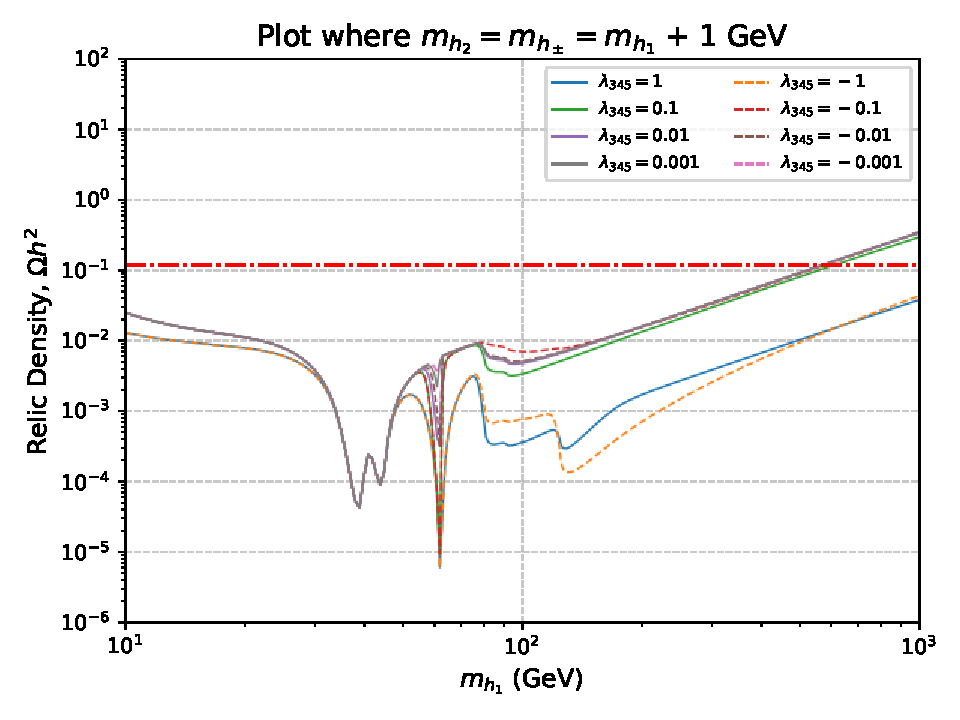
\includegraphics[width=\columnwidth]{scans/1-D_scans/Omegah2_MD1_l345_+1/plot_MD1_l345.pdf}
    \caption{Relic density against $m_{h_1}$, the case where $\Delta m^0 = 1$ GeV. The red shaded region is the area excluded by LEP, and the red line the upper limit of DM relic density (Eqn. \ref{eqn:DM relic density value}).}
    \label{fig:MD1_l345_1}
\end{figure}

\begin{figure}[H]
    \centering
    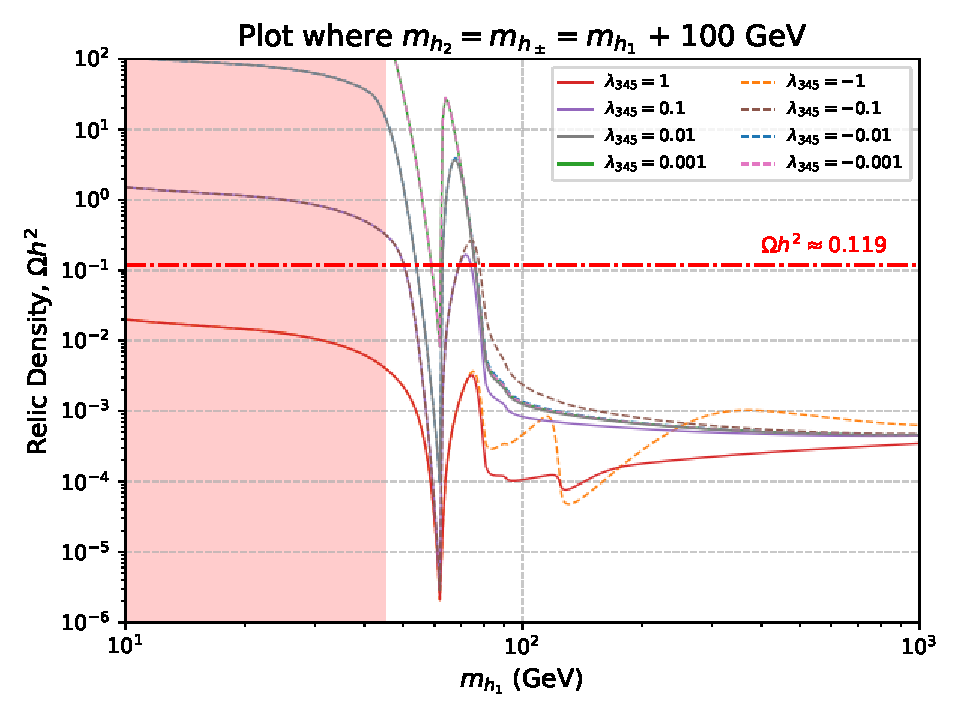
\includegraphics[width=\columnwidth]{plots/plot_MD1_l345+100.pdf}
    \caption{Relic density against $m_{h_1}$, the case where $\Delta m^0 = 100$ GeV}
    \label{fig:MD1_l345_100}
\end{figure}

In Fig. \ref{fig:MD1_l345_1} and \ref{fig:MD1_l345_100}, we alter the masses of the DM candidate, $h_1$ and its complementary particles ($h_2$ and $h_{\pm}$) to observe the relic density, we make a few observations:
\begin{itemize}
    \item The slight dips at 40 and 45 GeV for all values of $\lambda$ is the reaction where $h, h \rightarrow Z_0$ boson, and also the reaction for $h, h \rightarrow W_\pm$. The $Z^0$ and $W^\pm$ boson have masses $\sim$80 GeV and $\sim$85 GeV respectively.
    \item At 60 GeV, there is a dip for all values of $\lambda$ - this is because that is the $h_1,h_1\rightarrow H$ process - the DM DM annihilation process. 
    \item At 80-90 GeV
    \item At 105 GeV
\end{itemize}
\begin{figure}
    \centering
    \includegraphics[width=0.5\linewidth]{plots/}
    \caption{Caption}
    \label{fig:enter-label}
\end{figure}
\section{Analysis}
\label{sec:analysis}

\section{Conclusion}
\label{sec:conclusion}

\newpage
\bibliographystyle{plain}
\bibliography{references}

\end{document}

**Introduction**
The Higgs potential, characterized by a Mexican hat-shaped function, determines the vacuum expectation value (VEV) of the Higgs boson, denoted as $v$. The symmetry breaking of the degrees of freedom associated with the Higgs boson leads to the loss of these degrees of freedom to other baryons, resulting in the VEV.

We extend this concept to propose the existence of a new set of particles that follow a similar pattern. To achieve this, we impose a condition that the second doublet, denoted as $h_2$, is inert, meaning it does not share its degrees of freedom with other particles or couples to fermions.

The primary objective of this paper is to discover and analyze the parameters, namely $m_{h_1}$, $m_{h_2}$, $h_{h_\pm}$, $\lambda_2$, and $\lambda_{345}$, for the i2HDM model. In Section \ref{sec:i2HDM}, we provide a detailed introduction to the i2HDM model. Section \ref{sec:methodology} introduces the tools employed and the methods used to fix or scan the parameters. Section \ref{sec:results} presents the results obtained, followed by an analysis in Section \ref{sec:analysis}. Finally, the conclusion is presented in Section \ref{sec:conclusion}.